\section{Potencial eléctrico}
\label{sec:potencial}

Así como el concepto de trabajo y energía hizo posible resolver con facilidad algunos problemas de mecánica, el empleo de las ideas de energía también hace más fácil la solución de una variedad de problemas de electricidad.

Cuando una partícula con carga se mueve por un campo eléctrico, el campo ejerce una fuerza que efectúa trabajo sobre la partícula. Este trabajo siempre se puede expresar en términos de la energía potencial eléctrica. Así como la energía potencial gravitatoria depende de la altura de una masa sobre la superficie terrestre, la energía potencial eléctrica depende de la posición que ocupa la partícula con carga en el campo eléctrico. Describiremos la energía potencial eléctrica utilizando un concepto llamado \emph{potencial eléctrico} o simplemente potencial.

\begin{tcolorbox}[interesting_data]
  A modo de recordatorio, el trabajo \(W_{ab}\) realizado por una fuerza \(\vec{F}\) sobre una partícula para desplazarla desde el punto \(a\) al punto \(b\) se define como 
  \[
    W_{ab}=\int_a^b \vec{F}\cdot d\vec{s}
  \]
  Donde la fuerza \(\vec{F}:\mathbb{R}^3 \mapsto \mathbb{R}^3\) es una función vectorial o un campo vectorial que tiene como valores de entrada puntos. Es usual usar la notación \(\vec{F}(\vec{r})\) para indicar que \(\vec{F}\) depende del vector posición \(\vec{r}\), mientras que el desplazamiento \(d\vec{s}\) es el vector tangente de un diferencial de posición  del camino de integración. La fuerza y el vector desplazamiento se multiplican con el producto escalar, ya que la fuerza que actúa perpendicular respecto del desplazamiento no realiza trabajo. En definitiva, solo se toma la componente paralela de la fuerza al desplazamiento.

  Un campo, como puede ser el campo gravitatorio \(\vec{g}\) o el campo eléctrico \(\vec{E}\) se denominan campos conservativos. Un campo es conservativo si su rotacional es cero y cumple con el Teorema de Stokes (su dominio sea simplemente conexo). Esta afirmación no se demostrará pero es importante tenerla presente, ya que de a partir de esto puede demostrarse que 
  \begin{itemize}
    \item el trabajo realizado por una fuerza conservativa es independiente de la trayectoria,
    \item el trabajo es nulo si la trayectoria es cerrada (\(a=b\)), y
    \item siempre puede encontrarse una función potencial \(U\) tal que \(\vec{F}=-\nabla U\).
  \end{itemize}

  Si la fuerza \(\vec{F}\) es producida por un campo conservativo significa que la energía invertida en realizar un trabajo es almacenada en dicho campo. Aunque es conveniente aclarar que la energía no es únicamente del campo, más bien corresponde al sistema partícula-campo. A esta energía se la denomina energía potencial \(U\). Por ejemplo, si eleva una pelota, usted está realizando un trabajo sobre la misma, sin embargo si la suelta cae. Esto se debe a que parte de la energía fue almacenada en el sistema pelota-campo gravitatorio como energía potencial gravitatoria.

  Si usted desplaza la pelota a \textbf{velocidad constante} (sin aceleración) del punto \(a\) al punto \(b\), entonces el trabajo total \(W_{ab}=0\) ya que \(F_\text{aplicada}=-F_\text{peso}\) y \(\sum F_i = 0\), sin embargo su trabajo individual \(W_\text{ext}\) será igual pero opuesto al que realiza el campo \(-W_\text{int}\). En otras palabras, el cambio en la energía potencial almacenada por el campo gravitatorio será igual al trabajo que usted realizó que a su vez será igual (en magnitud) al trabajo que realizó el campo. A este trabajo que realiza el campo se le denomina \(W_\text{int}\), y puede calcularse como
  \[
    W_\text{int}= -\Delta U \quad \text{y, en consecuencia} \quad W_\text{ext}= \Delta U.
  \]
  De donde se puede concluir que si el trabajo \(W_\text{int}\) resulta positivo entonces la energía potencial en \(a\) es mayor que en \(b\). Es decir si mueve la pelota a velocidad constante hacia abajo (a favor del campo) la pelota pierde energía potencial, significa que la capacidad del campo para realizar trabajo en \(b\) es menor que en \(a\). En definitiva, la energía potencial del sistema disminuye y esa disminución es igual al trabajo positivo realizado por el campo.

  Por último, para terminar la revisión, recuerde el teorema del trabajo y la energía, que establece que el \emph{cambio} en la energía cinética \(\Delta K\) durante cualquier desplazamiento es igual al trabajo total realizado sobre la partícula. Si el único trabajo efectuado sobre la partícula lo realizan fuerzas conservativas, entonces 
  \[
    \Delta K = - \Delta U \qquad \Rightarrow \qquad K_a + U_a = K_b + U_b
  \]
  Es decir, la energía total inicial es igual a la energía total final. O en otras palabras, la energía mecánica total \(E_\text{mecánica} = K + U\) se conserva. Es decir todo trabajo de fuerzas conservativas es un intercambio de energía cinética y potencial.
\end{tcolorbox}

Volviendo con electrostática, cuando se coloca una carga de prueba \(q_0\) en un campo eléctrico \(\vec{E}\), la carga experimenta una fuerza eléctrica \(\vec{F_e}=q_0\vec{E}\). Esta fuerza es conservativa, lo que significa que el trabajo realizado por la fuerza al mover la carga entre dos puntos \(A\) y \(B\) no depende de la trayectoria seguida, sino solo de los puntos inicial y final.

El trabajo realizado por la fuerza al mover la carga \(q_0\) desde el punto \(A\) hasta el punto \(B\) se define como
\begin{equation*}
  W_{AB} = \int_A^B \vec{F_e} \cdot d\vec{s} = \int_A^B q_0\vec{E} \cdot d\vec{s}
\end{equation*}
Y como la fuerza eléctrica es conservativa, podemos expresarla en términos de la energía potencial eléctrica \(U\),
\begin{equation*}
  W_{AB} = U_A - U_B = -\Delta U = \int_A^B \underbrace{q_0\vec{E}}_{\vec{F}_e} \cdot d\vec{s}
\end{equation*}
\begin{tcolorbox}[myconclusion]
  Recuerde que la fuerza es una función, por tanto es lo que se busca integrar.
\end{tcolorbox}
Entonces, para el trabajo realizado por una fuerza eléctrica, lo que importa es cómo varía la fuerza a lo largo del desplazamiento. Como la fuerza eléctrica es una fuerza conservativa, el trabajo no depende de la trayectoria seguida por la carga de prueba \(q_0\), sino únicamente de la diferencia de energía potencial entre las posiciones inicial y final del trayecto.

La energía potencial eléctrica \(U\) del sistema depende de la configuración espacial de las cargas. Para deducir su valor absoluto, es necesario establecer un punto de referencia donde la energía potencial sea cero. En el caso de un campo generado por una carga puntual \(q\), es conveniente establecer este nivel cero en el infinito, donde las cargas están tan alejadas que no interactúan. 

\begin{marginfigure}
  \centering
  \caption{Gráfica de la energía potencial \(U\) de dos cargas puntuales contra su separación \(r\).}
  \label{fig_funcion_energia_potencial}
  \begin{tikzpicture}[>=stealth]
  \begin{axis}[
      axis lines = middle, 
      xlabel={$r$},
      ylabel={$U$},
      ymin=-0.5, ymax=6.5,
      xmin=-0.5, xmax=6.5,
      xtick=\empty,
      ytick=\empty,
      domain=0.17:5.5, 
      samples=100,
      grid=none,
      width=\marginparwidth,
      height=\marginparwidth,
      axis line style={gray}
    ]
    \addplot[teal, very thick] {1/x};
  \end{axis}
  \shade[ball color=orange] (1,2) circle (.15) node[above=1mm] {\scriptsize$q$};
  \shade[ball color=orange] (2,2) circle (.15) node[above=1mm] {\scriptsize$q_0$};
  \draw[thin] (1,1.8) -- (1,1.6);
  \draw[thin] (2,1.8) -- (2,1.6);
  \draw[thin,<->] (1,1.7) -- node[below] {$r$} (2,1.7);
  \shade[ball color=blue!40] (1,2.7) circle (.15) node[above=1mm] {\scriptsize$q$};
  \shade[ball color=blue!40] (2,2.7) circle (.15) node[above=1mm] {\scriptsize$q_0$};
\end{tikzpicture}
\vspace{1cm}
\begin{tikzpicture}[>=stealth]
  \begin{axis}[
      axis lines = middle, 
      xlabel={$r$},
      ymin=-6.5, ymax=0.5,
      xmin=-0.5, xmax=6.5,
      xtick=\empty,
      ytick=\empty,
      domain=0.17:5.5, 
      samples=100,
      grid=none,
      width=\marginparwidth,
      height=\marginparwidth,
      axis line style={gray}
    ]
    \addplot[teal, very thick] {-1/x};
  \end{axis}
  \shade[ball color=blue!40] (1,1) circle (.15) node[above=1mm] {\scriptsize$q$};
  \shade[ball color=orange] (2,1) circle (.15) node[above=1mm] {\scriptsize$q_0$};
  \draw[thin] (1,0.8) -- (1,0.6);
  \draw[thin] (2,0.8) -- (2,0.6);
  \draw[thin,<->] (1,0.7) -- node[below] {$r$} (2,0.7);
  \shade[ball color=orange] (1,1.7) circle (.15) node[above=1mm] {\scriptsize$q$};
  \shade[ball color=blue!40] (2,1.7) circle (.15) node[above=1mm] {\scriptsize$q_0$};
  \node (cartel) [
    text width=3cm,
    align=left,
    fill=yellow!40!black!14,
    draw=yellow!40!black!46,
    thick,
    rounded corners=2pt,
    inner sep=2mm
    ]
    at (1.35,-2) {\footnotesize{Cuando las cargas son iguales, el potencial es mayor si la distancia es menor. Lo contrario ocurre cuando son distintas.}};
\end{tikzpicture}

\end{marginfigure}
De esta forma, la energía potencial \(U\) del sistema formado por una carga fuente \(q\) y una carga de prueba \(q_0\) separadas por una distancia \(r\), equivale al trabajo realizado por un agente externo para traer la carga de prueba desde el infinito hasta dicha distancia \(r\) sin aceleración:
\[
  U = k_e\frac{q q_0}{r}~ [\unit{\joule}]
\]
donde \(r\) es la distancia entre la carga de prueba \(q_0\) y la carga fuente \(q\).

Como se puede intuir, este punto de referencia de energía potencial cero depende de la configuración de cargas y del campo; si bien suele fijarse en el infinito para cargas puntuales (como muestra la figura \ref{fig_funcion_energia_potencial}), en otros sistemas prácticos puede convenir fijarlo en otro lugar, como en la superficie de un conductor o en la ``tierra''.

\subsection{Definición de potencial eléctrico}

\begin{definition}[Potencial Eléctrico]\label{def_potencial}
Para una posición conocida de la carga de prueba en el campo, el sistema carga-campo tiene una energía potencial \(U\) relativa a la configuración del sistema definida como \(U=0\). Al dividir la energía potencial entre la carga de prueba \(q_0\), obtenemos el \emph{potencial eléctrico} \(V\) en un punto \(P\) del campo eléctrico:
\begin{equation}
  V = \frac{U}{q_0} ~ [\unit{\joule\per\coulomb}]
  \label{eq:potential}
\end{equation}
\end{definition}

El potencial eléctrico es una magnitud escalar que se mide en \unit{\volt} (voltios)\footnote{Observe el importante detalle tipográfico, el potencial eléctrico se denota con una \(V\) mayúscula itálica, mientras que la unidad voltio se denota con una \unit{\volt} mayúscula regular.} y se define como la energía potencial por unidad de carga.
% En versiones futuras, se podría usar \(\mathcal{V}\) en vez de V, para evitar confusión.

Teniendo en cuenta la definición \ref{def_potencial} de potencial y la ecuación \eqref{eq:potential}, se define la diferencia de potencial \(\Delta V = V_B - V_A\) entre dos puntos \(A\) y \(B\) en un campo eléctrico. Esto representa el cambio de energía potencial por unidad de carga al mover una carga de prueba \(q_0\) entre esos dos puntos
\begin{equation}
  \Delta V = \frac{\Delta U}{q_0} = -\int_A^B \vec{E} \cdot d\vec{s}
  \label{eq:potential_difference}
\end{equation}

Por la ecuación \eqref{eq:potential_difference}, el trabajo realizado por un agente externo al desplazar una carga \(q\) a través de un campo eléctrico con una velocidad constante es:
\[
  W=q\Delta V
\]

Es muy importante que el desplazamiento de la carga \(q\) sea a velocidad constante, ya que si no lo es, el trabajo realizado por el agente externo no será igual al trabajo realizado por la fuerza eléctrica. 

\begin{tcolorbox}[myconclusion]
  Cuando se habla de un agente externo y desplazamiento a velocidad constante (o sin aceleración) es importante entender que se busca que \(\Delta K = 0\). De esta forma el trabajo total que es el cambio en la energía cinética más el cambio en la energía potencial resultará 
  \[
    W = \Delta U + \cancel{\Delta K}
  \]
\end{tcolorbox}
\begin{figure}[!ht]
  \centering
  \begin{subfigure}[b]{0.45\textwidth}
    \centering
    \begin{tikzpicture}[>=stealth]
      \coordinate (A) at (0,1);
      \coordinate (B) at (0,-1);
      \begin{scope}[very thick,decoration={
          markings,
          mark=at position 0.6 with {\arrow{>}}
        }] 
        \foreach \x in {-1,-.5,...,1} {
          \draw[orange, thick,postaction=decorate] (\x,1.5) -- (\x,-1.5);
        }
      \end{scope}
      \shade[ball color=orange, opacity=0.3, text opacity=1] (A) circle (.2) node[left=1mm] {\scriptsize{A}};
      \shade[ball color=orange] (B) circle (.2) node[left=1mm] {\scriptsize{B}};
      \draw[thin] ($(A)+(0.4,0)$) -- ($(A)+(0.9,0)$);
      \draw[thin] ($(B)+(0.4,0)$) -- ($(B)+(0.9,0)$);
      \draw[thin,<->] ($(A)+(.75,0)$) -- node[fill=white,inner sep=1pt] {$d$} ($(B)+(.75,0)$);
      \node at (-1.3,-1) {$\vec{E}$};

      \node (cartel) [
        font=\footnotesize,
        text width=4.5cm,
        align=left,
        fill=yellow!40!black!14,
        draw=yellow!40!black!46,
        thick,
        rounded corners=2pt,
        inner sep=2mm
        ]
        at ($(A)+(0,1.7)$) {Cuando una carga de prueba positiva se mueve del punto A al punto B, la energía potencial eléctrica del sistema carga-campo disminuye.};
    \end{tikzpicture}
  \end{subfigure}
  \begin{subfigure}[b]{0.45\textwidth}
    \centering
    \begin{tikzpicture}[>=stealth]
      \coordinate (A) at (0,1);
      \coordinate (B) at (0,-1);
      \begin{scope}[very thick,decoration={
          markings,
          mark=at position 0.6 with {\arrow{>}}
        }] 
        \foreach \x in {-1,-.5,...,1} {
          \draw[blue!50, thick,postaction=decorate] (\x,1.5) -- (\x,-1.5);
        }
      \end{scope}
      \shade[ball color=blue!50, opacity=0.3, text opacity=1] (A) circle (.2) node[left=1mm] {\scriptsize{A}};
      \shade[ball color=blue!50] (B) circle (.2) node[left=1mm] {\scriptsize{B}};
      \draw[thin] ($(A)+(0.4,0)$) -- ($(A)+(0.9,0)$);
      \draw[thin] ($(B)+(0.4,0)$) -- ($(B)+(0.9,0)$);
      \draw[thin,<->] ($(A)+(.75,0)$) -- node[fill=white,inner sep=1pt] {$d$} ($(B)+(.75,0)$);
      \node at (-1.3,-1) {$\vec{g}$};

      \node (cartel) [
        font=\footnotesize,
        text width=4.5cm,
        align=left,
        fill=yellow!40!black!14,
        draw=yellow!40!black!46,
        thick,
        rounded corners=2pt,
        inner sep=2mm
        ]
        at ($(A)+(0,1.7)$) {Cuando un objeto con masa se mueve del punto A al punto B, la energía potencial gravitacional del sistema objeto-campo disminuye.};
    \end{tikzpicture}
  \end{subfigure}
  \caption{Comparación de la energía potencial eléctrica y gravitatoria.}
  \label{fig_potential_uniform}
\end{figure}


Nótese que el concepto de potencial eléctrico se concibe de forma similar al de campo eléctrico. Se usa una carga de prueba positiva \(q\) haciendo que sólo dependa de la carga fuente \(Q\) que genera el campo eléctrico. 

\subsection{Diferencia de potencial en un campo eléctrico uniforme}

La ecuación \eqref{eq:potential_difference} es válida en todos los campos eléctricos, sean uniformes o no, es decir, es la fórmula general para la obtención de la diferencia de potencial. Sin embargo, en un campo eléctrico uniforme, la magnitud del campo \(\vec{E}\) es constante y la dirección de \(\vec{E}\) es la misma en todos los puntos del campo, de modo tal que se pueden simplificar los cálculos. En este caso, la diferencia de potencial entre dos puntos \(A\) y \(B\) separados por una distancia \(d\) en la dirección del campo eléctrico se puede expresar como:
\begin{equation}
  \Delta V = -\int_A^B \vec{E} \cdot d\vec{s} = -E \, \int_A^B ds = \boxed{-Ed}
  \label{eq:potential_uniform}
\end{equation}
donde \(E\) es la magnitud del campo eléctrico y \(d\) es la distancia entre los puntos \(A\) y \(B\) en la dirección del campo.

El signo negativo indica que el potencial en el punto \(B\) es menor que el potencial en el punto \(A\) si la carga de prueba se mueve en la dirección del campo eléctrico. Esto significa que el trabajo realizado por la fuerza eléctrica es negativo, lo que implica que la energía potencial disminuye al mover la carga en la dirección del campo eléctrico.

\begin{tcolorbox}[mydanger]
  Atención, si la carga \(q\) es negativa, la situación se invierte. El sistema gana energía potencial al mover la carga \(q\) en la dirección del campo eléctrico, y disminuye al moverla en la dirección opuesta.    
\end{tcolorbox}

\subsection{Potencial eléctrico en un punto}

\begin{marginfigure}
  \centering
  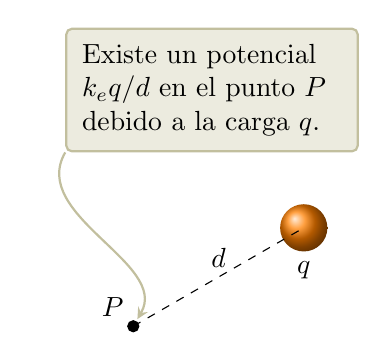
\begin{tikzpicture}[>=stealth]
    \coordinate (P) at (0,0);
    \shade[ball color=orange] (30:2.5) circle (.3) node[below=3mm] {$q$};
    \draw[dashed] (P) -- node[above] {$d$} (30:2.5);
    \filldraw (P) circle (2pt) node[above left] {$P$};
    \node (cartel) [
      text width=3.3cm,
      align=left,
      fill=yellow!40!black!14,
      draw=yellow!40!black!46,
      thick,
      rounded corners=2pt,
      inner sep=2mm
      ]
      at (1,3) {Existe un potencial $k_e q/d$ en el punto $P$ debido a la carga $q$.};
    \draw[->, thick, color=yellow!40!black!46, shorten >=3pt] 
             (cartel.south west) to[out=240, in=60] (P);
  \end{tikzpicture}
  \caption{Potencial en el punto \(P\) debido a \(q\).}
  \label{fig_potencial_en_un_punto}
\end{marginfigure}


Como se mencionó previamente, la energía potencial \(U\) es relativa a un punto que se ha definido como punto de potencial cero. Esto es importante ya que la definición de potencial eléctrico \(V\) parte del concepto de energía potencial, por cuanto, hereda estos comportamientos. Esto implica que si usted desea conocer el potencial en un punto \(P\) como muestra la figura \ref{fig_potencial_en_un_punto}, entonces primero debe saber cual es el punto de potencial cero\footnote{El potencial en un punto es simplemente un caso especial de la diferencia de potencial, donde el punto de partida (usualmente el infinito para cargas puntuales) tiene un potencial de \qty{0}{\volt}.}. De este modo, la distancia de \(P\) a dicho punto de potencial cero, dará la diferencia de potencial de \(P\) con respecto al punto de potencial cero, y consecuentemente, el potencial de \(P\). Entonces el potencial \(V\) en el punto \(P\) es el trabajo requerido para mover la carga de prueba desde el infinito hasta el punto \(P\). Aplicando la definición de potencial, el potencial en el punto \(P\) se obtiene de la siguiente manera,
\begin{align*}
    V_P &= - \lim_{a \to \infty}\int_{a}^d \vec{E} \cdot d\vec{r}\\
        &= - \lim_{a \to \infty}\int_{a}^d \frac{kq}{r^2} \cdot dr\\
        &= -kq \, \lim_{a \to \infty} \int_{a}^d \frac{1}{r^2} \cdot dr\\
        &= -kq \, \lim_{a \to \infty} \left[ -\frac{1}{r} \right]_{a}^d\\
        &= -kq \, \lim_{a \to \infty} \left[ -\frac{1}{d} + \frac{1}{a} \right]\\
        &= -kq \, \left[ -\frac{1}{d} + 0 \right] \\
    V_P &= k\frac{q}{d} = \lVert\vec{E}\rVert \, \lVert\vec{r}\rVert \cos(0)
\end{align*}
siendo \(\lVert \vec{r}\rVert\) el radiovector de módulo \(d\) que apunta a \(P\). Por ser \(\vec{E}\) y \(\vec{r}\) paralelos. Entonces el potencial eléctrico en un punto \(P\) debido a una carga puntual \(q\) es:
\begin{equation}
    \boxed{V_P = k\frac{q}{d} = E \, d}
    \label{eq:potential_point_charge}
\end{equation}
donde \(q\) es la carga fuente, \(E\) el campo generado por \(q\) y \(d\) la distancia al punto \(P\).

El potencial eléctrico debido a múltiples cargas puntuales se basa en el principio de superposición, que establece que el potencial eléctrico total en un punto es igual a la suma algebraica de los potenciales individuales producidos por cada carga.
\begin{equation}
    V_\text{total} = \sum_{i=1}^{n} V_i = k \sum_{i=1}^{n} \frac{q_i}{d_i}
\end{equation}

\subsection{Obtención de \texorpdfstring{\(\vec{E}\)}{E} a partir de \texorpdfstring{\(V\)}{V}}

El campo eléctrico \(\vec{E}\) y el potencial eléctrico \(V\) están relacionados, como se muestra en la ecuación \eqref{eq:potential_point_charge}, que se usa para encontrar \(V\) en un punto cuando se conoce \(\vec{E}\). Aunque, también podemos encontrar \(\vec{E}\) a partir de \(V\) usando la relación:
\begin{equation}
  dV = -\vec{E} \cdot d\vec{s}
  \label{eq:field_from_potential_differential}
\end{equation}
y si estamos trabajando con una única coordenada (por ejemplo, un movimiento rectilíneo) podemos escribir la ecuación \eqref{eq:field_from_potential_differential} como:
\[
  dV = -E \, ds \quad \Rightarrow \quad E = -\frac{dV}{ds}
\]

Sin embargo, en general, el potencial eléctrico es una función de las tres coordenadas espaciales. Si \(V(r)\) se da en coordenadas cartesianas, las componentes \((E_x, E_y, E_z)\) del campo eléctrico pueden ser determinadas fácilmente a partir de \(V(x, y, z)\) como derivadas parciales
\begin{equation}
  \boxed{
    \vec{E} = -\nabla V
  }
\end{equation}
donde \(\nabla\) es el operador nabla, que representa el gradiente del potencial eléctrico. Esta relación indica que el campo eléctrico es igual al negativo del gradiente del potencial eléctrico. En otras palabras, el campo eléctrico apunta en la dirección de mayor disminución del potencial eléctrico.

\begin{tcolorbox}[interesting_data,title=Recordatorio]
El operador nabla \(\nabla\) (u operador del gradiente) es una herramienta matemática usada en cálculo vectorial y análisis multivariable. Se utiliza para representar derivadas en múltiples dimensiones.

Formalmente, el operador nabla se define como:
\[
\nabla = \left( \frac{\partial}{\partial x}, \frac{\partial}{\partial y}, \frac{\partial}{\partial z} \right)
\]
Es un operador vectorial que, aplicado a diferentes tipos de funciones, da lugar a distintos conceptos. En nuestro caso solo vamos a repasar el concepto de gradiente.

Cuando se aplica el operador nabla a una función escalar \( f(x, y, z) \), produce un campo vectorial que apunta en la dirección de mayor incremento de la función. Se expresa como:
\[
\nabla f = \left( \frac{\partial f}{\partial x}, \frac{\partial f}{\partial y}, \frac{\partial f}{\partial z} \right)
\]
Este vector resultante indica la dirección en la que la función crece más rápidamente y su magnitud corresponde a la tasa de cambio máxima. En el caso de \(\vec{E}\) y \(V\), \(\vec{E}\) es el gradiente de \(V\) representa una función vectorial que apunta en la dirección de mayor aumento del potencial eléctrico.
\end{tcolorbox}

\begin{comment}
  Siento que todo el apartado de potencial eléctrico no se entiende bien. Es decir, conceptualmente, las derivaciones de fórmulas son claras. Sin embargo el concepto de potencial siento que no está bien explicado. Voy a dejar algunos comentarios al respecto.


  Punto número 1: debería demostrar que la fuerza eléctrica (dada por la fuerza de Coulomb) es una fuerza conservativa.
  Punto número 2: Esta unidad se llama electrostática, hay que dejar bien claro que se busca relacionar el trabajo interno (realizado por el campo) con el potencial eléctrico. El potencial eléctrico, en esencia, es el trabajo realizado por el campo al mover una partícula de un punto A a otro B. Por eso, \Delta K debe ser cero. El agente externo cumple ese rol: decirnos que trabajo efectúa el campo. Será positivo si se aleja (siendo del mismo signo) y negativo si se acerca. ¿por que? El campo genera fuerza opuesta si me acerco (quiere expulsarla) y me ayuda si me alejo (porque quiere expulsarla).

  De el punto 2 saca una conclusión, partiendo de la definición. Si $W=-\Delta U$ y $V=U/q$, luego $W=-\Delta V/q = \int_A^B q\vec{E}d\vec{s}$. Esto lleva a 
  $$
  V=-\int_A^B \vec{E}d\vec{s}
  $$
  Que es la relación que existe entre el campo y el potencial. ¿Por qué negativo? Si yo quiero ir en contra del campo (me acerco) tengo que aumentar el potencial; es decir, hacer trabajo, ya que el trabajo que hace el campo sobre mi intención de movimiento es negativo (en mi contra).
  Si el potencial en A es mayor que el potencial en B significa que he perdido potencial, o en otras palabras, capacidad de realizar trabajo. Esto es porque el campo empuja con menos fuerza, ya que la fuerza decrece con el cuadrado de la distancia.

  Una posible alternativa para abordar este tema es de forma ``incremental''. Primero analizamos una carga fuente puntual, la carga de prueba $q_0$ y la distancia en un único eje de movimiento (el eje x). En este caso particular entonces se ve claramente la relación de distancia y potencial. 

  Luego, podemos abordar el caso en donde el campo $\vec{E}$ es uniforme, usando el típico caso de las placas planas paralelas. Esto lleva a la típica fórmula de $-Ed$. 

  Por último, vemos el caso donde $\vec{E}$ y $q$ están en el plano y $\vec{E}$ es un campo vectorial de cualquier forma. Entonces, en este caso, debemos aplicar la fórmula de la integral de un campo vectorial (que no es lo mismo que la integral de línea usual), para al final, con el teorema de green demostrar que se puede resolver como una integral doble, que podemos relacionar con una integral de línea.???
  
  Tenemos que el trabajo es 
  $$
  W = \int_A^B \vec{F}\cdot d\vec{s}
  $$
  Con $d\vec{s}$ un diferencial de desplazamiento. El producto escalar ¿Por que? porque solo la fuerza actúa en la dirección del desplazamiento. 
  Digamos supongamos que queremos empujar una caja. Si la fuerza la aplicamos justo para adelante, entonces toda la fuerza actuará en ese trabajo. Si por otro lado, empujamos a 45 grados, tenemos que la fuerza vertical actúa, pero no hay desplazamiento, entonces no hay trabajo. Horizontalmente solo se aplica una parte de la fuerza, que corresponde a $F\cos(45)$. Y para que sea igual al trabajo, lo multiplicamos por el desplazamiento.
  $$
  W = F s \cos(45)
  $$
  O en otras palabras: $W=\vec{F}\cdot\vec{s}$ donde $\vec{s}$ es el vector desplazamiento. ¿Qué es el desplazamiento? Recuerda! es la diferencia de los vectores posición. Y para que el desplazamiento sea igual a la trayectoria, tenemos que debemos tomar pequeños diferenciales de desplazamiento. Entonces, pasamos por todos y cada uno de los vectores posición que modelan la trayectoria de la carga.

  Respecto de mi relación con el teorema de green, debo analizar bien esto, porque es un lío. Dejaré otro comentario respecto a mi duda y luego la respuesta de la IA.
\end{comment}
\begin{comment}
  Tengo una duda. Digamos que tenemos un campo vectorial (como $\vec{E(x,y)}$) que a cada punto, asigna un vector (tal como el campo eléctrico). Entonces la fuerza que siente una carga de prueba q es $q\vec{E}$. En consecuencia, si quiero integrar
  $$
  V=-\int_A^B q\vec{E}d\vec{s}
  $$
  Donde $\vec{s}$ es un vector tangente a la trayectoria realizada por $q$. Esto ¿Se puede ver como una integral de línea? Según puedo entender, para un campo vectorial tenemos que la integral sobre el campo es una integral particular que podemos relacionar a una integral doble en una región de dos funciones $M$ y $N$ de dos variables. Esto no es una integral de línea usual sinó más bien una integral de un campo vectorial, que podemos resolver usando el teorema de green. ¿Por qué tomamos que $\vec{E}(x,y)$ es una función escalar para integrarla usando una integral de línea?

  ¿Estoy muy confundido o más o menos bien encaminado?

  -- 

¡Vas por un camino excelente! No estás confundido, estás en esa fase de "conexión de cables" donde la física se encuentra con el cálculo multivariable, y es normal que surjan estas dudas sobre la naturaleza de las integrales.

Vamos a desenredar esos conceptos, porque tienes la intuición correcta pero algunos términos se están cruzando.

---

### 1. ¿Es una integral de línea?

**Sí, absolutamente.** Lo que planteas es la definición de una **integral de línea de un campo vectorial**.

Hay una pequeña precisión técnica en tu fórmula: el potencial eléctrico  se define como la energía por unidad de carga. Por tanto, la carga  no va dentro de la integral de . La relación es:

* **Trabajo ():** 
* **Diferencia de Potencial ():** 

### 2. ¿Por qué parece que "integramos un escalar"?

Aquí está la clave de tu duda: **el producto punto**.
Un campo vectorial  no se puede integrar directamente de forma "lineal" porque es un vector. Para poder sumarlo a lo largo de una trayectoria (una integral es una suma infinita), necesitamos convertirlo en un número (escalar) en cada punto.

Al hacer el producto punto , estamos proyectando el campo eléctrico sobre la dirección del movimiento:


Lo que terminas integrando es  (donde  y ). Esto **sigue siendo una integral de línea**, pero de un campo vectorial. No es que tratemos a  como un escalar, es que el producto punto *lo convierte* en la componente escalar que realiza trabajo en esa dirección.

### 3. El Teorema de Green y los Campos Conservativos

Mencionaste el **Teorema de Green**, y aquí es donde tu razonamiento se vuelve muy potente. Green relaciona una integral de línea en una **curva cerrada** con una integral doble en el área que encierra:


En electrostática (cargas en reposo), el campo eléctrico es **conservativo**. Esto significa que:

1. Su rotacional es cero: , lo que implica que .
2. Según el Teorema de Green, si la curva es cerrada, ¡la integral es cero!
3. Esto implica que la integral **no depende del camino**, solo de los puntos inicial  y final .

Por eso, en el ejercicio anterior, simplemente multiplicamos . Como el campo es uniforme y la trayectoria es recta, la integral de línea se simplifica a una multiplicación básica, pero "escondida" hay una integral de línea donde el ángulo entre  y  es constante.

### Resumen de tu "mapeo mental":

* **Integral de línea usual (escalar):** Integras una función (como la densidad de un cable) sobre una curva. .
* **Integral de línea de campo vectorial:** Integras la componente tangencial de un campo (como el trabajo). . **Esta es la que usamos en física.**
* **Teorema de Green:** Es una herramienta para resolver estas integrales en 2D cuando la trayectoria vuelve al origen, pero no es la definición de la integral en sí.

¿Te hace sentido ver el producto punto como el "traductor" de vector a escalar para poder integrar? Si quieres, podemos ver cómo se aplicaría esto si el campo eléctrico no fuera uniforme, sino que dependiera de la posición (como el de una carga puntual).
\end{comment}

\begin{comment}
  Hola Elio. Es un excelente avance para el libro de Física 2. La estructura general del documento en LaTeX es muy prolija, y el nivel de rigor matemático es el adecuado, aprovechando bien los conceptos de cálculo vectorial (como integrales de línea y gradientes) para formalizar la teoría.

He analizado el texto y, en términos generales, las deducciones y definiciones son sólidas. Sin embargo, he notado dos detalles importantes, uno pedagógico y otro conceptual, que deberías corregir antes de continuar:

### 1. Confusión entre campo uniforme y campo de una carga puntual

En la sección **Potencial eléctrico en un punto**, al final del desarrollo de la integral, llegas a la siguiente conclusión:



Y luego lo encuadras como:


**El error:** Pedagógicamente, igualar el potencial de una carga puntual a  es muy peligroso. Matemáticamente es una tautología si evalúas la magnitud del campo  *exactamente* en el punto a una distancia  (ya que ), pero conceptualmente invita al lector a confundir este caso con la fórmula del campo eléctrico uniforme (). En una carga puntual, el campo no es constante a lo largo del trayecto desde el infinito hasta , por lo que la relación lineal  no describe el proceso físico de esa integración.

**Sugerencia:** Elimina la equivalencia con  y el producto escalar de esa línea. Quédate únicamente con el resultado de la integral: .

### 2. Contradicción en la dirección del gradiente

En la subsección **Obtención de  a partir de **, explicas correctamente en el texto principal que el campo eléctrico apunta en la dirección de mayor *disminución* del potencial eléctrico ().

**El error:** En el cuadro `tcolorbox` de Recordatorio, escribes:

> *"En el caso de  y ,  es el gradiente de  representa una función vectorial que apunta en la dirección de mayor aumento del potencial eléctrico."*

Aquí te faltó considerar el signo negativo. El gradiente de  () efectivamente apunta hacia donde el potencial aumenta más rápido. Pero como el campo eléctrico es el gradiente *negativo* (), este apunta exactamente en la dirección opuesta: hacia donde el potencial **disminuye** más rápido.

---

Corrigiendo esos dos detalles, el texto base queda impecable. Ahora bien, mencionaste que estás teniendo serios problemas de interpretación con respecto al potencial eléctrico.

¿Cuál es la duda o el obstáculo conceptual específico que te está frenando? ¿Te gustaría que lo analicemos paso a paso?
\end{comment}
